% Put the project details here

\section{PROJECT DETAILS}

\subsection{Overview}

The \textit{Digital Farmers' Produce System} is a cloud-based web application developed to support agricultural coordination and market linkages in the Municipality of Sinacaban, Misamis Occidental. The system provides a centralized platform where farmers can post available produce, buyers can view and inquire about crop listings, and agriculture personnel can monitor basic crop information and farmer support requests.

The system connects four main groups of users:

\begin{itemize}
    \item \textbf{Farmers} can manage their produce listings, indicate available quantities and harvest information, communicate with buyers, submit requests for farming resources such as seeds, fertilizers, or other assistance, and receive important updates through system notifications or SMS alerts.
    
    \item \textbf{Buyers} can browse, search, and filter available products, view produce details, and contact farmers for possible offline transactions.
    
    \item \textbf{Agriculture Officers} can monitor crop listings, review barangay-level stock information, respond to resource requests, publish advisories, send notifications, and generate simple summaries for decision-making.
    
    \item \textbf{Administrators} can manage user accounts, system records, and basic configuration settings.
\end{itemize}

The system is deployed in a shared cloud hosting environment and is accessible through desktop and mobile web browsers. Its design considers the local context of Sinacaban, including intermittent internet connectivity, limited technical resources, and varying levels of digital literacy among users. To improve accessibility, the system includes SMS notification support and a Bisaya language toggle for users who prefer localized interface text.

\subsection{Project Framework}

\begin{figure}[htbp]
    \centering
    \vspace{4ex}
    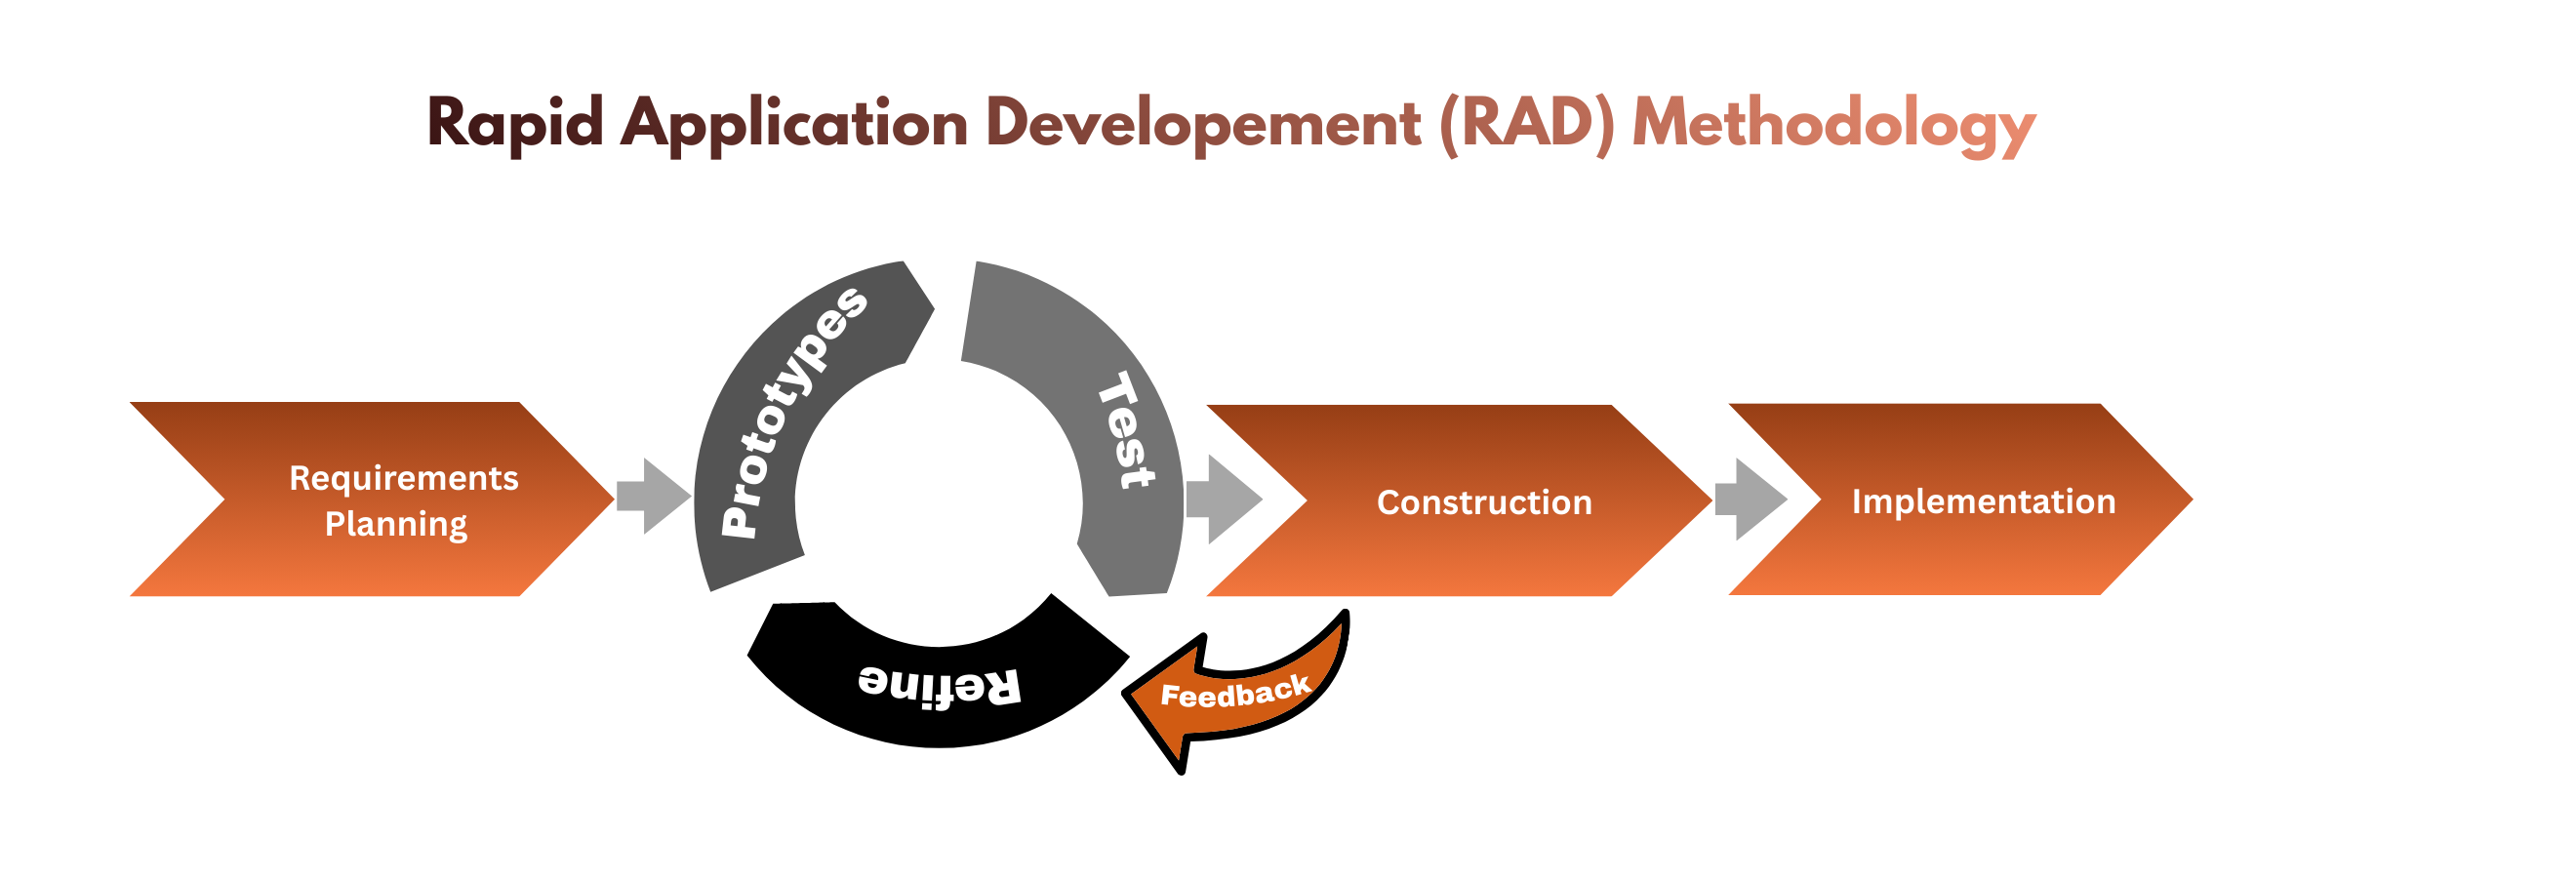
\includegraphics[width=0.85\textwidth]{Texfiles/Picture/Picture.png}
    \caption{Rapid Application Development (RAD)}
    \label{fig:rad-framework}
\end{figure}

The project used the Rapid Application Development (RAD) framework as the guiding methodology for the design, development, and evaluation of the \textit{Digital Farmers' Produce System}. RAD emphasizes rapid prototyping, iterative development, and active user feedback throughout the system development process \citep{Martin1991}. This approach was appropriate for the project because the system needed to respond to the practical needs of farmers, buyers, and agriculture personnel while allowing adjustments based on user feedback.

\subsubsection*{Phases of the RAD Framework}

The project followed the four major phases of the RAD framework:

\begin{enumerate}
    \item \textbf{Requirements Planning} -- Data were gathered from farmers, buyers, and agriculture personnel through interviews, surveys, and review of existing agricultural coordination practices. This phase identified the main problems, user needs, functional requirements, non-functional requirements, and limitations of the project.
    
    \item \textbf{User Design} -- Wireframes, mockups, and user flows were prepared to visualize the main system processes. These included user registration, login, produce posting, buyer searching, messaging, resource request submission, notification viewing, language selection, SMS notification support, and monitoring by agriculture personnel.
    
    \item \textbf{Construction} -- The web application was developed using the selected technologies and system design. Core modules such as user management, produce listing, buyer search, messaging, notifications, SMS alerts, resource requests, dashboard summaries, Bisaya language toggle, and CSV reporting were implemented and refined through testing and feedback.
    
    \item \textbf{Cutover} -- The system was prepared for pilot use and evaluation in the Municipality of Sinacaban. This phase included deployment to the cloud hosting environment, user orientation, user testing, security testing, bug fixing, and documentation of results.
\end{enumerate}

\subsection{System Models}

\subsubsection{Infrastructure Architecture}

\begin{figure}[htbp]
    \centering
    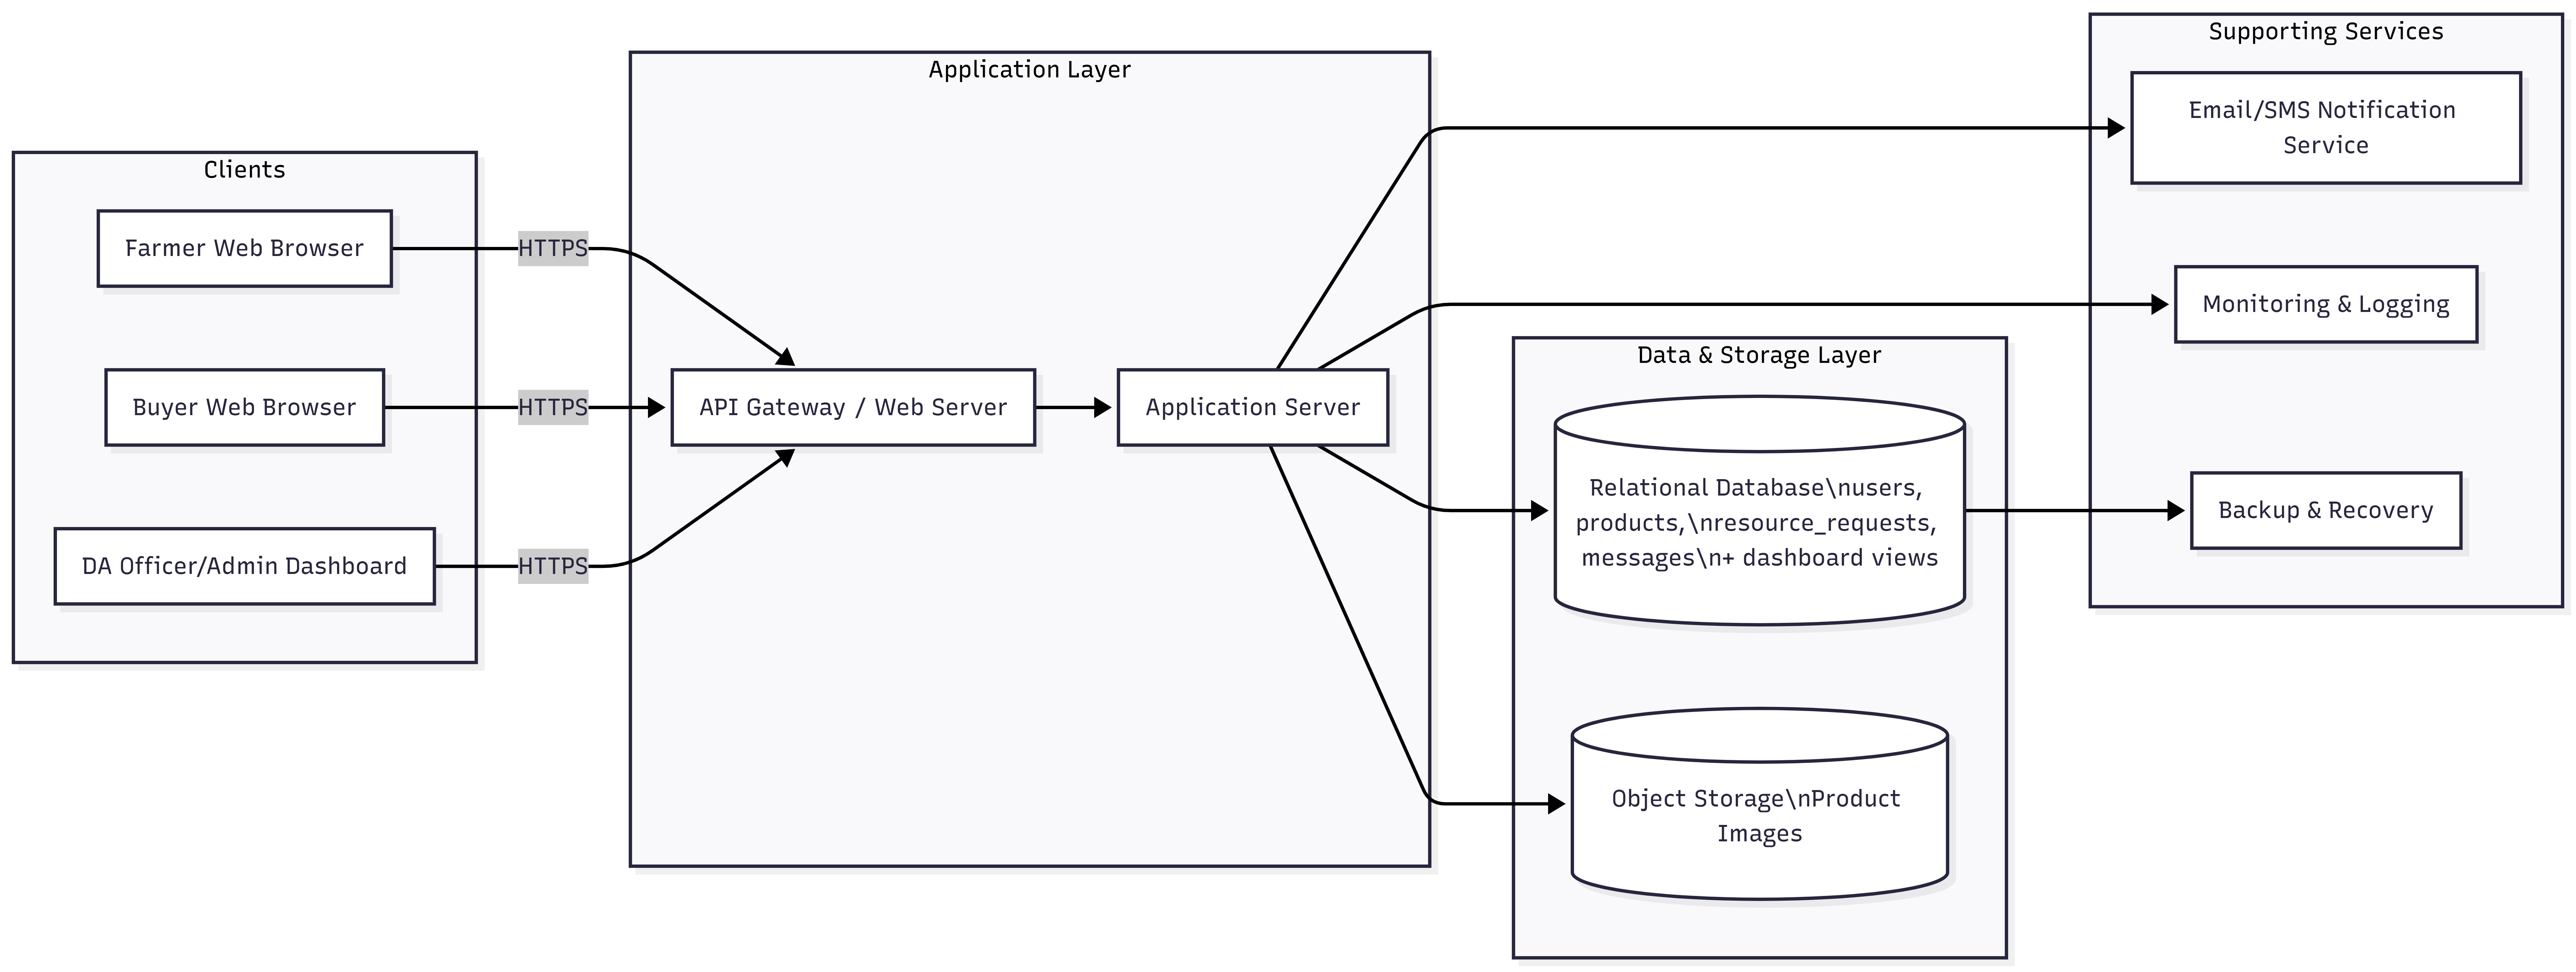
\includegraphics[width=0.9\textwidth]{Picture/infra.png}
    \caption{Infrastructure Architecture}
    \label{fig:infra-architecture}
\end{figure}

Figure~\ref{fig:infra-architecture} shows how the \textit{Digital Farmers' Produce System} is deployed and accessed by its users. Farmers, buyers, agriculture officers, and administrators use standard desktop or mobile web browsers to access the system through a secure HTTPS connection. Their requests pass through the web and application server, which manages user sessions, input validation, role-based access, and core business logic.

The system uses a cloud-hosted MySQL database to store structured information such as user accounts, produce listings, product categories, messages, notifications, resource requests, language settings, and system records. Product images and other uploaded files are stored and managed through the hosting environment. SMS notification support is integrated to send important updates, such as request status changes and advisories, to selected users. Regular backups and basic hosting monitoring support availability and data recovery.

This architecture supports centralized management, easier maintenance, and online accessibility for users in the municipality. It also allows the system to be used on common devices such as smartphones, laptops, and desktop computers.

\subsubsection{Entity Relationship Diagram}

\begin{figure}[htbp]
    \centering
    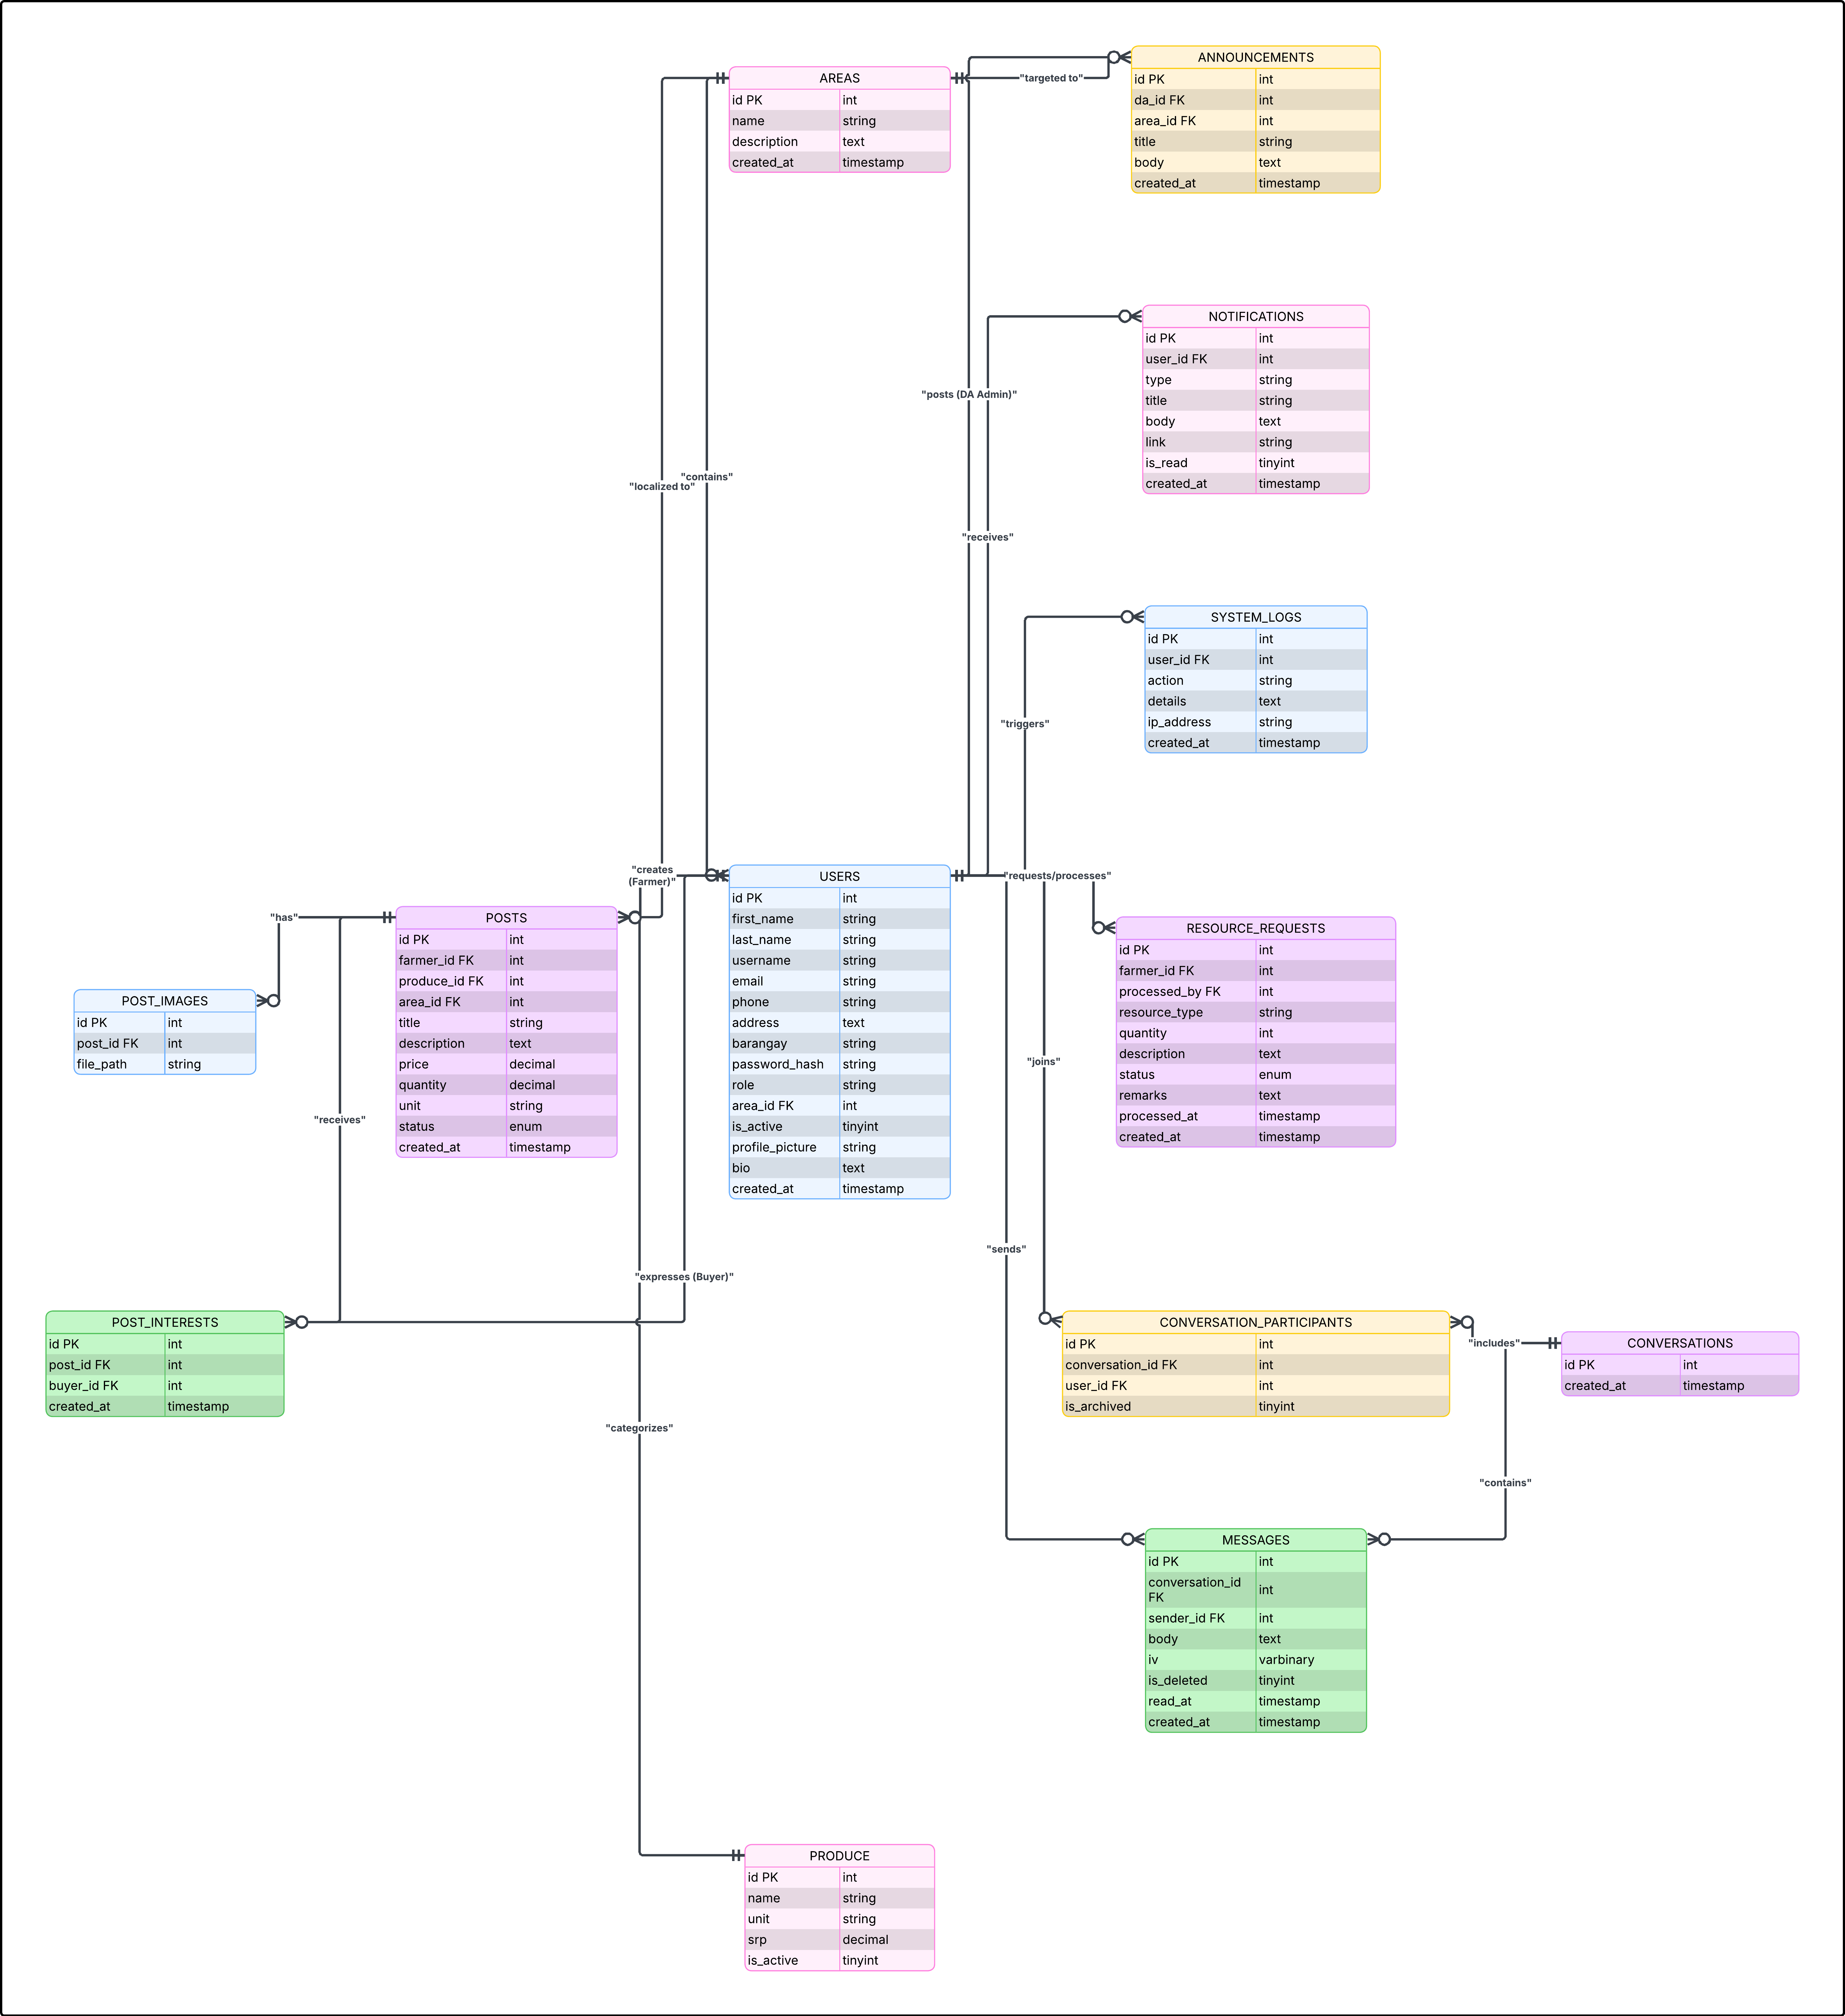
\includegraphics[width=0.9\textwidth]{Picture/erd.png}
    \caption{Entity Relationship Diagram}
    \label{fig:erd-logical}
\end{figure}

Figure~\ref{fig:erd-logical} presents the logical data model of the system. The central \textit{users} table stores account information and is connected to several core entities. A farmer can create multiple product listings, and each product listing belongs to a product category for standard classification. The \textit{messages} table records communication between users by identifying the sender and receiver of each message.

The \textit{resource\_requests} table records requests submitted by farmers for farming assistance. Agriculture officers are linked to the processing and updating of these requests. The system also supports notification-related records for system alerts and SMS updates. Summary or reporting views provide aggregated information, such as total available quantity per category and the number of pending, approved, or rejected requests. This data model supports produce management, communication, resource request processing, notification delivery, and agricultural monitoring.

\subsubsection{Use Case Diagram}

\begin{figure}[htbp]
    \centering
    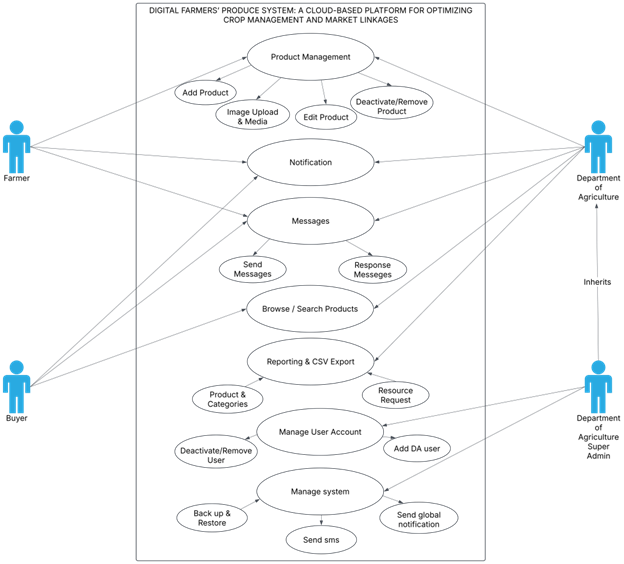
\includegraphics[width=0.9\textwidth]{Picture/ucd.png}
    \caption{Use Case Diagram}
    \label{fig:usecase}
\end{figure}

Figure~\ref{fig:usecase} summarizes the main functions available to each user role. Farmers can register, log in, manage produce listings, upload product images, send and receive messages, receive notifications, receive SMS alerts, use the Bisaya language option, and submit resource requests. Buyers can register, browse and search available products, view listing details, contact farmers, receive notifications, and use the language toggle where supported.

Agriculture officers can monitor farmer and buyer records, manage resource requests, respond to messages, send announcements or notifications, trigger SMS updates, and generate reports or CSV exports. Administrators handle user account management and system configuration. These use cases show how the system supports coordination among farmers, buyers, and the Municipal Agriculture Office.

\subsubsection{Context Diagram}

\begin{figure}[htbp]
    \centering
    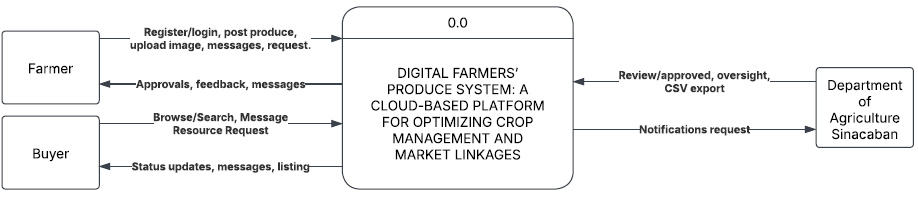
\includegraphics[width=0.9\textwidth]{Picture/context.png}
    \caption{Context Diagram}
    \label{fig:context}
\end{figure}

Figure~\ref{fig:context} gives a high-level view of the \textit{Digital Farmers' Produce System} as a single process interacting with external users. Farmers provide registration details, product posts, images, messages, resource requests, and language preferences. Buyers provide registration details, browsing and search requests, and messages. Agriculture officers provide review decisions, advisories, monitoring inputs, request updates, and notification content.

In return, the system provides product listings, request status updates, messages, system notifications, SMS alerts, localized interface labels, summaries, and downloadable reports. The diagram defines the system boundary and shows how information moves between the application and its users.

\subsubsection{Data Flow Diagram}

\begin{figure}[htbp]
    \centering
    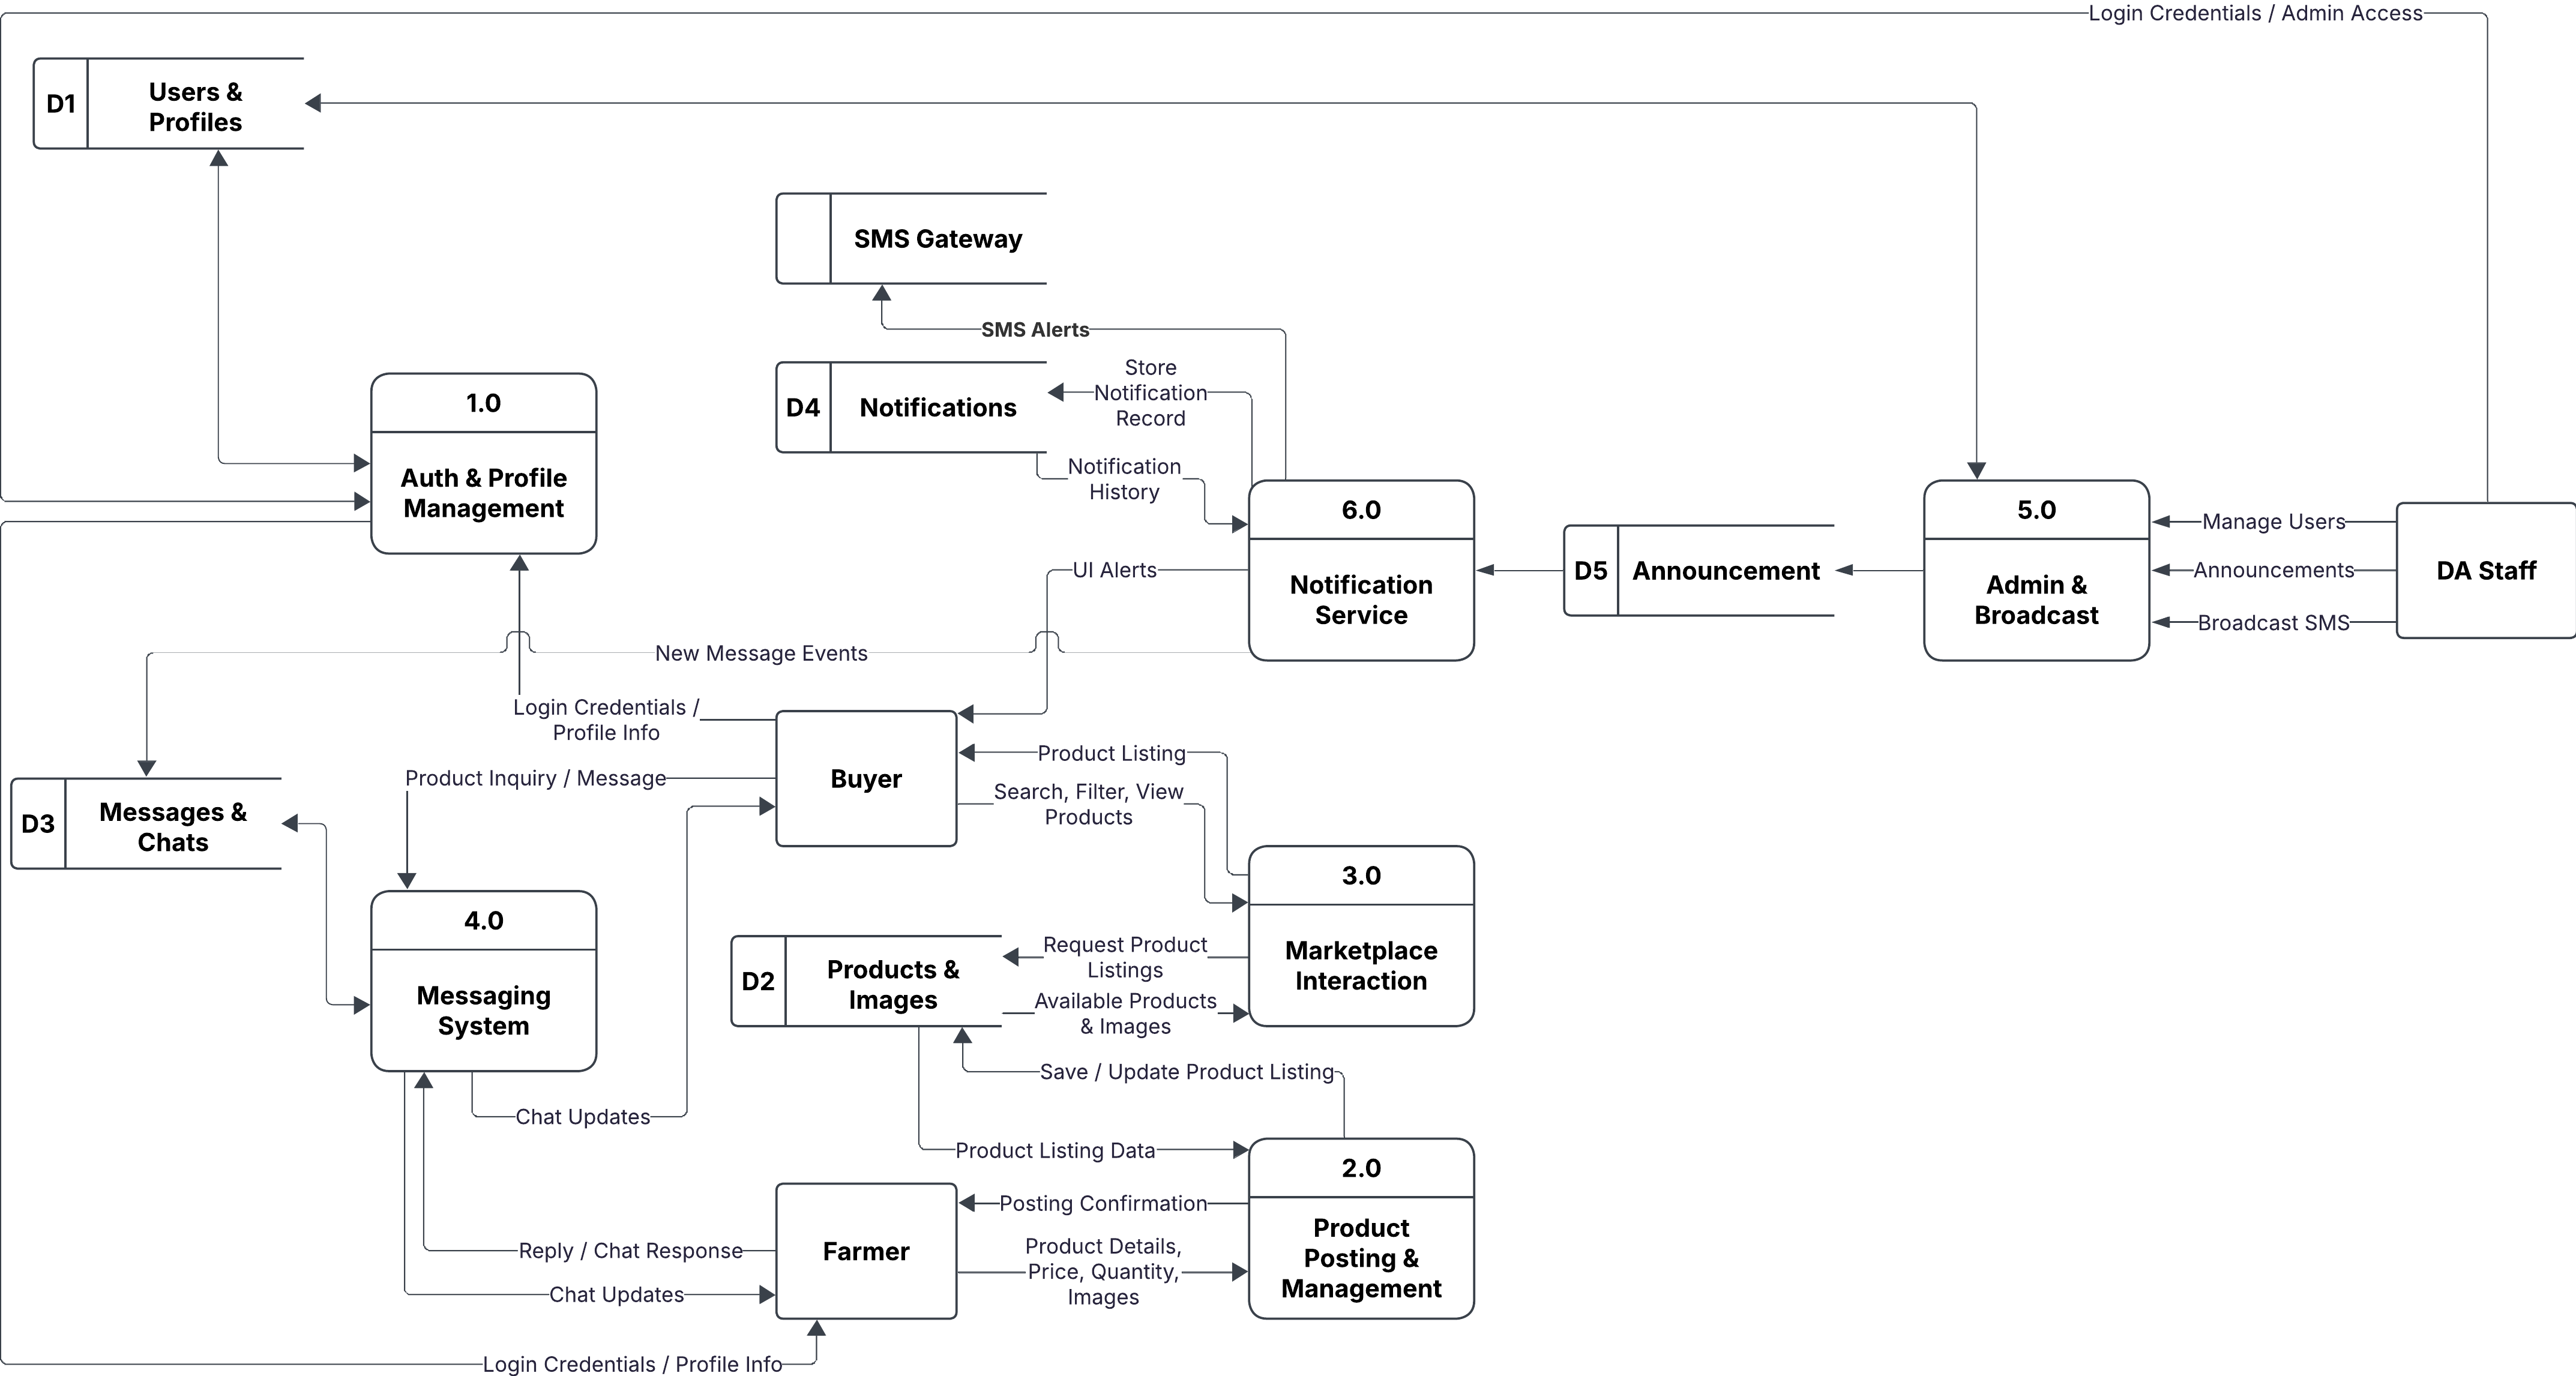
\includegraphics[width=0.9\textwidth]{Picture/dfd.png}
    \caption{Data Flow Diagram}
    \label{fig:dfd}
\end{figure}

Figure~\ref{fig:dfd} decomposes the system into major internal processes and data stores. The authentication and session process validates user credentials and manages access to the system. The product management process handles the creation, editing, viewing, and deactivation of produce listings. The request workflow process manages the submission, review, approval, or rejection of farmer resource requests.

The notification process records and delivers alerts and announcements to users. The SMS notification process sends selected important updates, such as resource request status and advisories, to farmers through text messages. The language toggle process supports the display of selected interface labels and instructions in Bisaya. The image upload and media process manages uploaded product images. The reporting and CSV export process retrieves relevant data from the system and generates summaries or downloadable reports. These processes show how user inputs are stored, processed, and returned as useful information.

\subsubsection*{Wireframes}

\subsubsection{Login Page}

\begin{figure}[htbp]
    \centering
    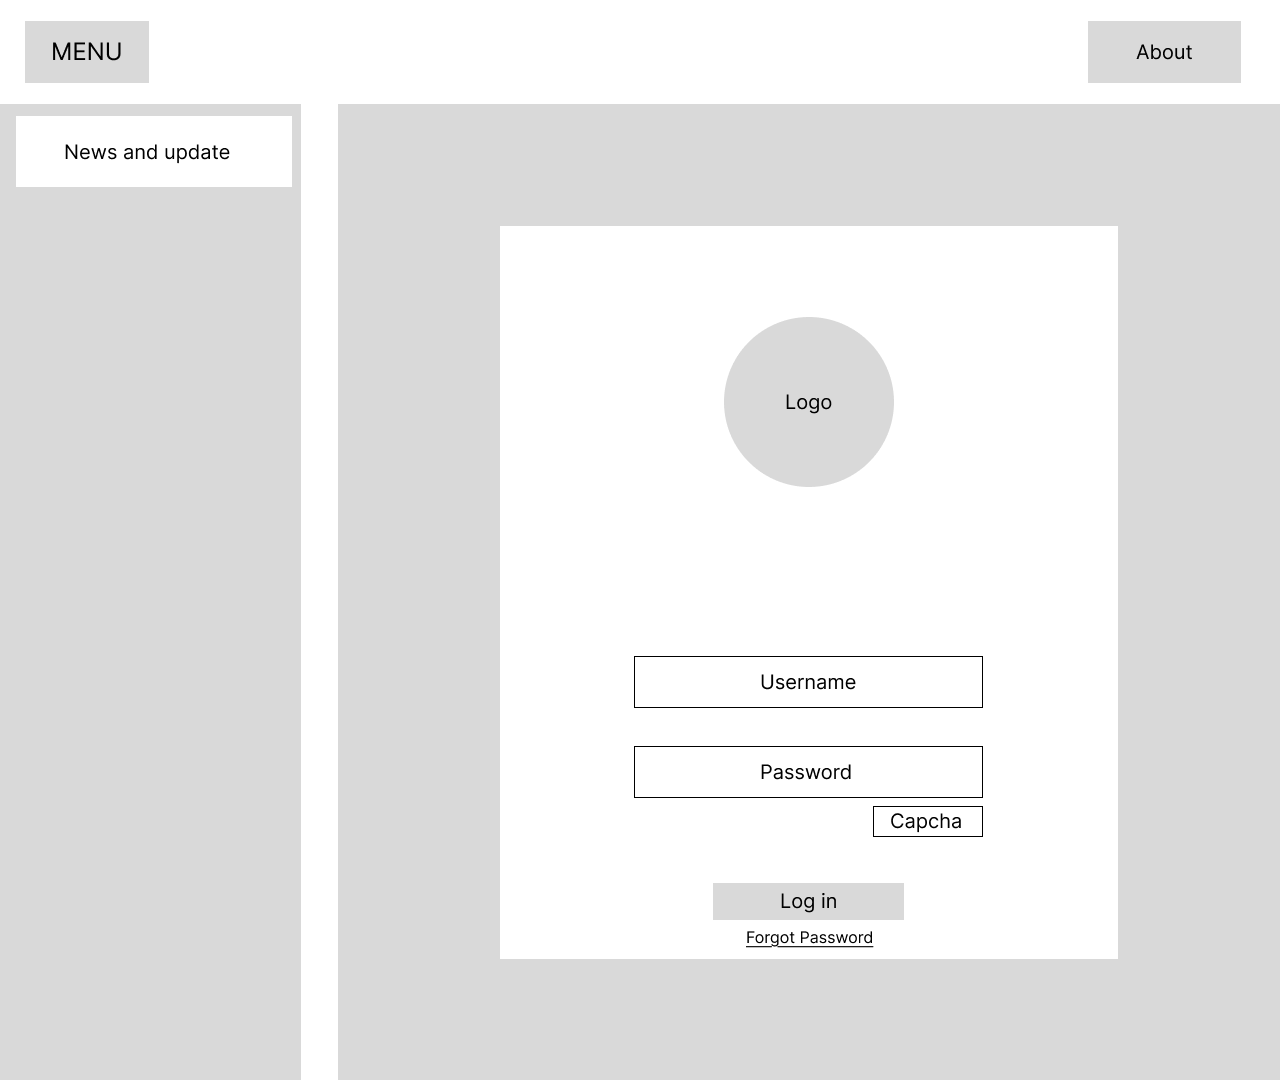
\includegraphics[width=0.9\textwidth]{Texfiles/images/wireframe/1. Login Page.png}
    \caption{Login Form}
    \label{fig:login-form}
\end{figure}

Figure~\ref{fig:login-form} shows the login page wireframe. The form contains fields for username, password, and captcha verification to help prevent automated login attempts. The \emph{Log in} button submits the user credentials, while the \emph{Forgot Password} option supports account recovery. The \emph{About} button provides basic information about the system for first-time users. The interface also supports localized labels through the Bisaya language toggle.

\subsubsection{Registration Page}

\begin{figure}[htbp]
    \centering
    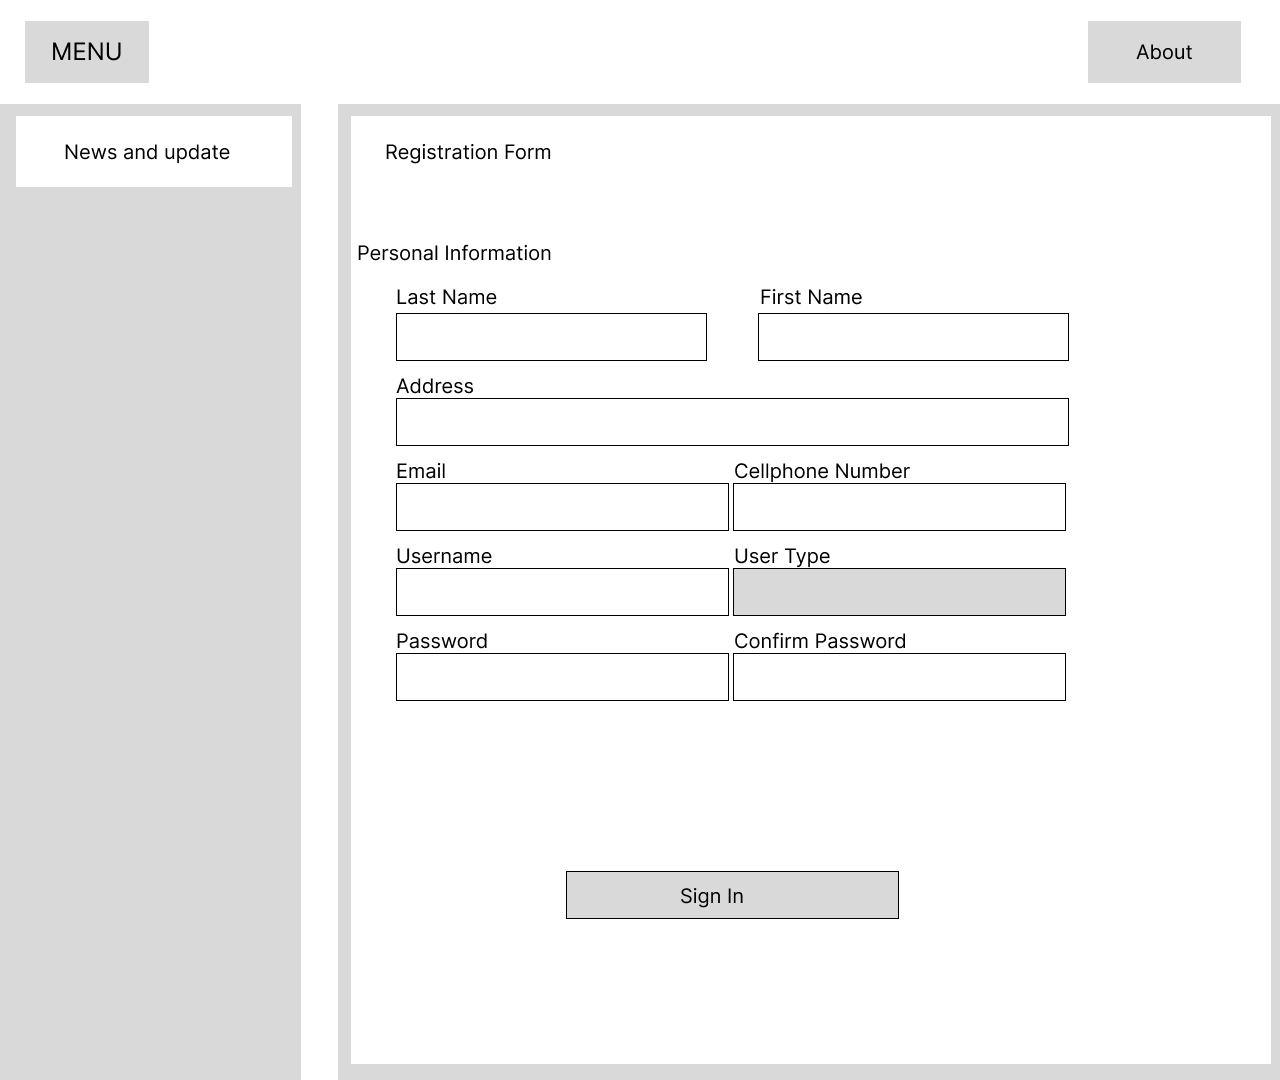
\includegraphics[width=0.9\textwidth]{Texfiles/images/wireframe/1.1 Registration.png}
    \caption{Registration Form}
    \label{fig:registration-form}
\end{figure}

Figure~\ref{fig:registration-form} shows the registration page used by new users to create an account. It collects basic information such as last name, first name, address, email address, cellphone number, username, password, and user type. The cellphone number is also used for SMS notification support when important updates need to be sent to the user. The system uses the registration information to assign the correct role and provide access to the appropriate functions.

\subsubsection{Farmer Home Page}

\begin{figure}[htbp]
    \centering
    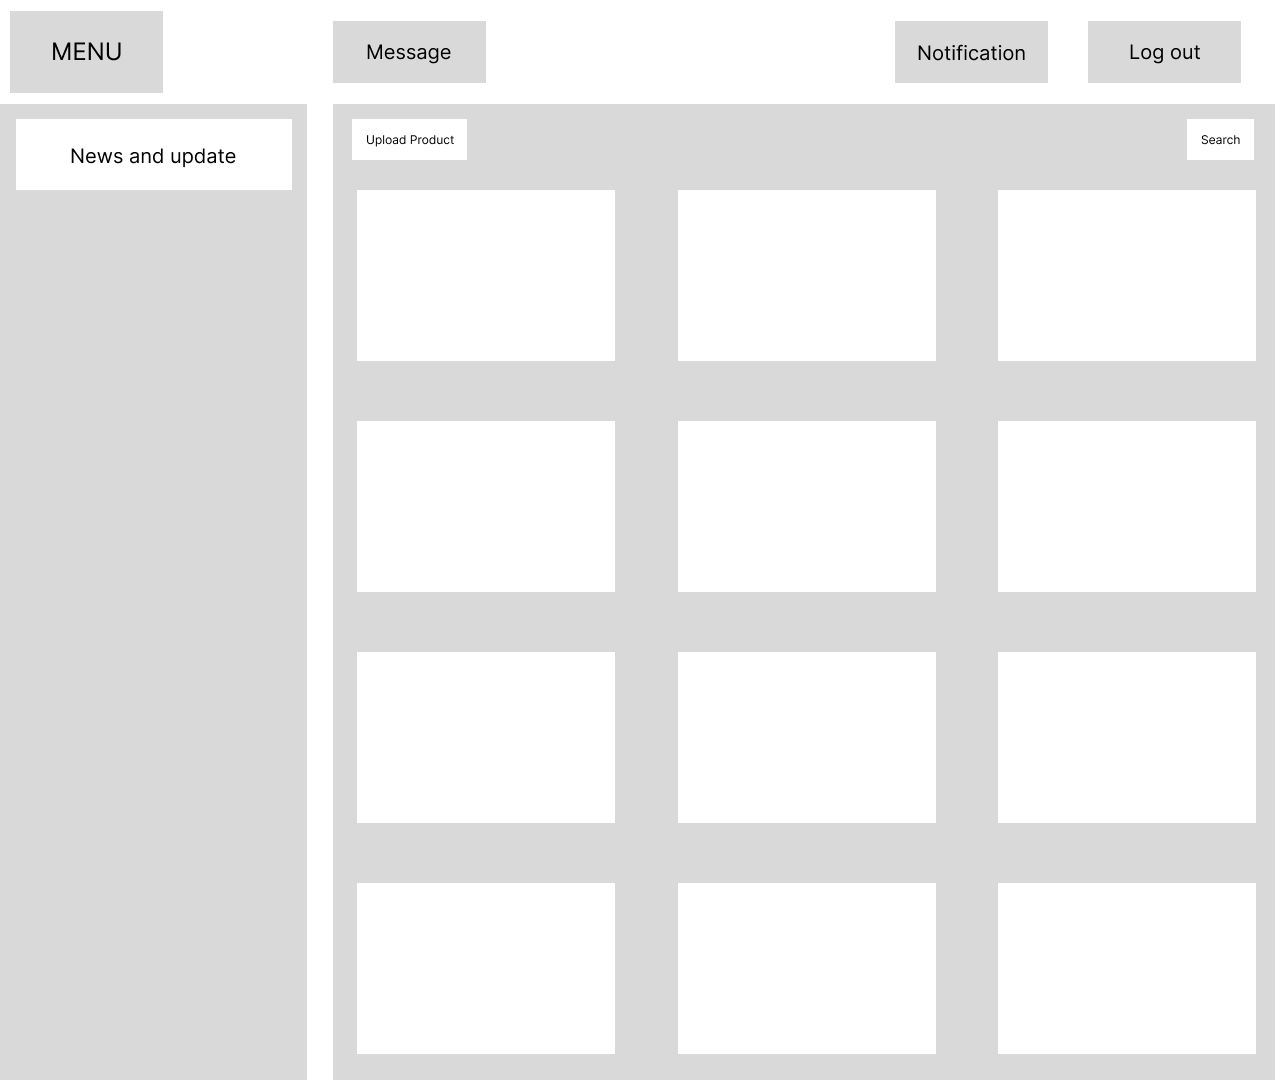
\includegraphics[width=0.9\textwidth]{Texfiles/images/wireframe/2. Farmers Home Page.png}
    \caption{Farmer Home Page}
    \label{fig:farmer-home}
\end{figure}

Figure~\ref{fig:farmer-home} shows the farmer home page. The main area displays product cards representing the farmer's uploaded produce. Farmers can add new listings, edit existing listings, search their products, and manage posted crop information such as price, quantity, location, and harvest details. Farmers can also receive system notifications and SMS alerts for important updates from the agriculture office.

\subsubsection{Buyer Home Page}

\begin{figure}[htbp]
    \centering
    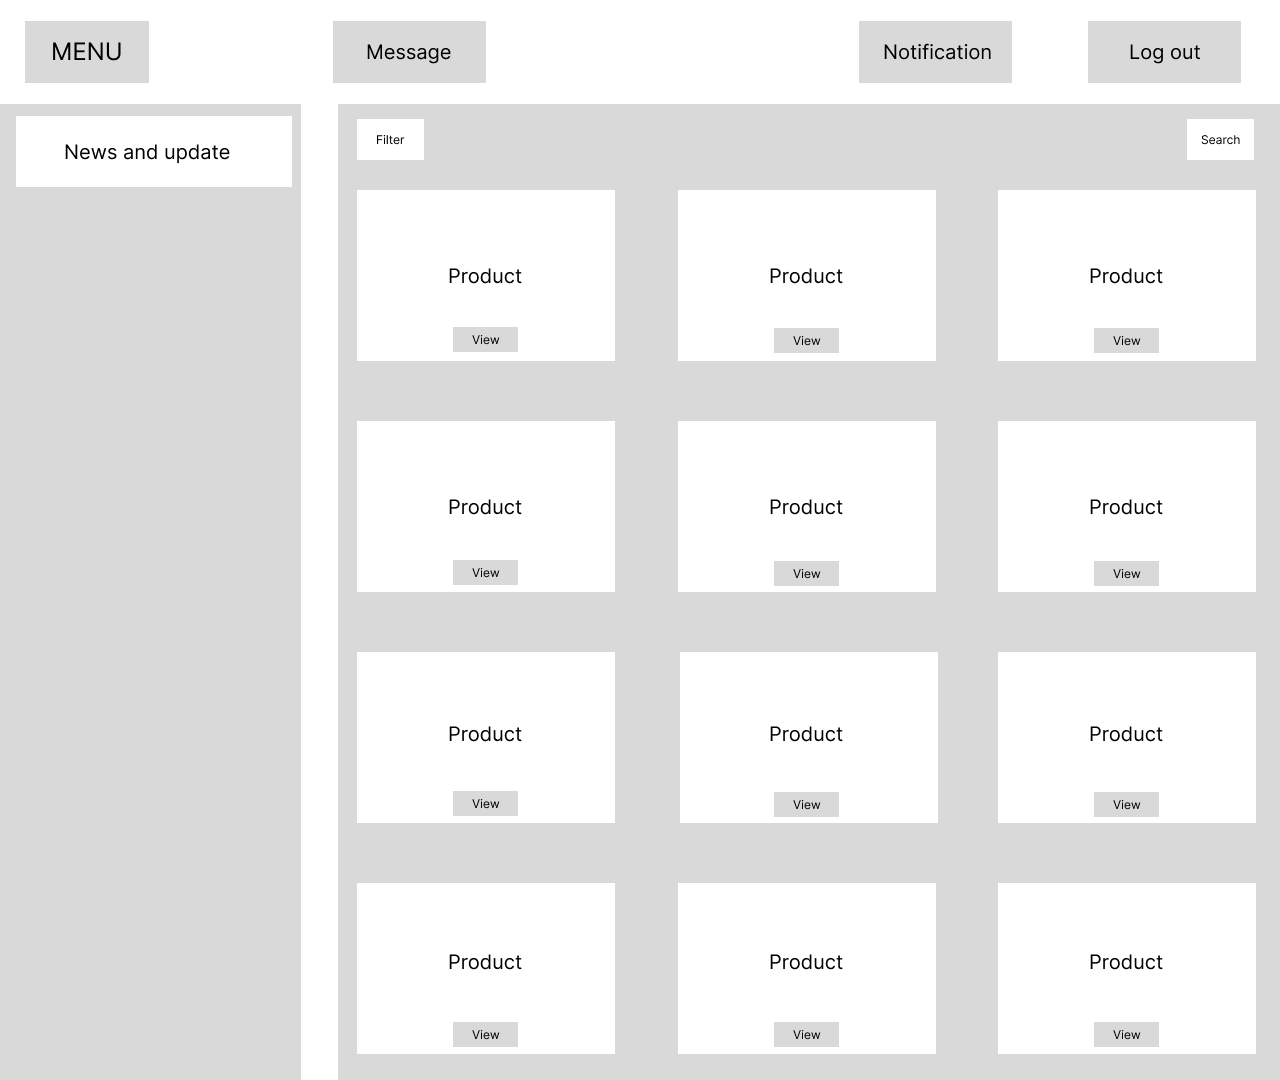
\includegraphics[width=0.9\textwidth]{Texfiles/images/wireframe/2.1 Buyer Home Page.png}
    \caption{Buyer Home Page}
    \label{fig:buyer-home}
\end{figure}

Figure~\ref{fig:buyer-home} shows the buyer home page. Buyers can browse available products using a grid or card layout. Each product card provides access to details such as crop name, price, quantity, farmer information, and contact options. The search and filter functions help buyers find products based on crop type, location, or availability.

\subsubsection{Agriculture Officer Home Page}

\begin{figure}[htbp]
    \centering
    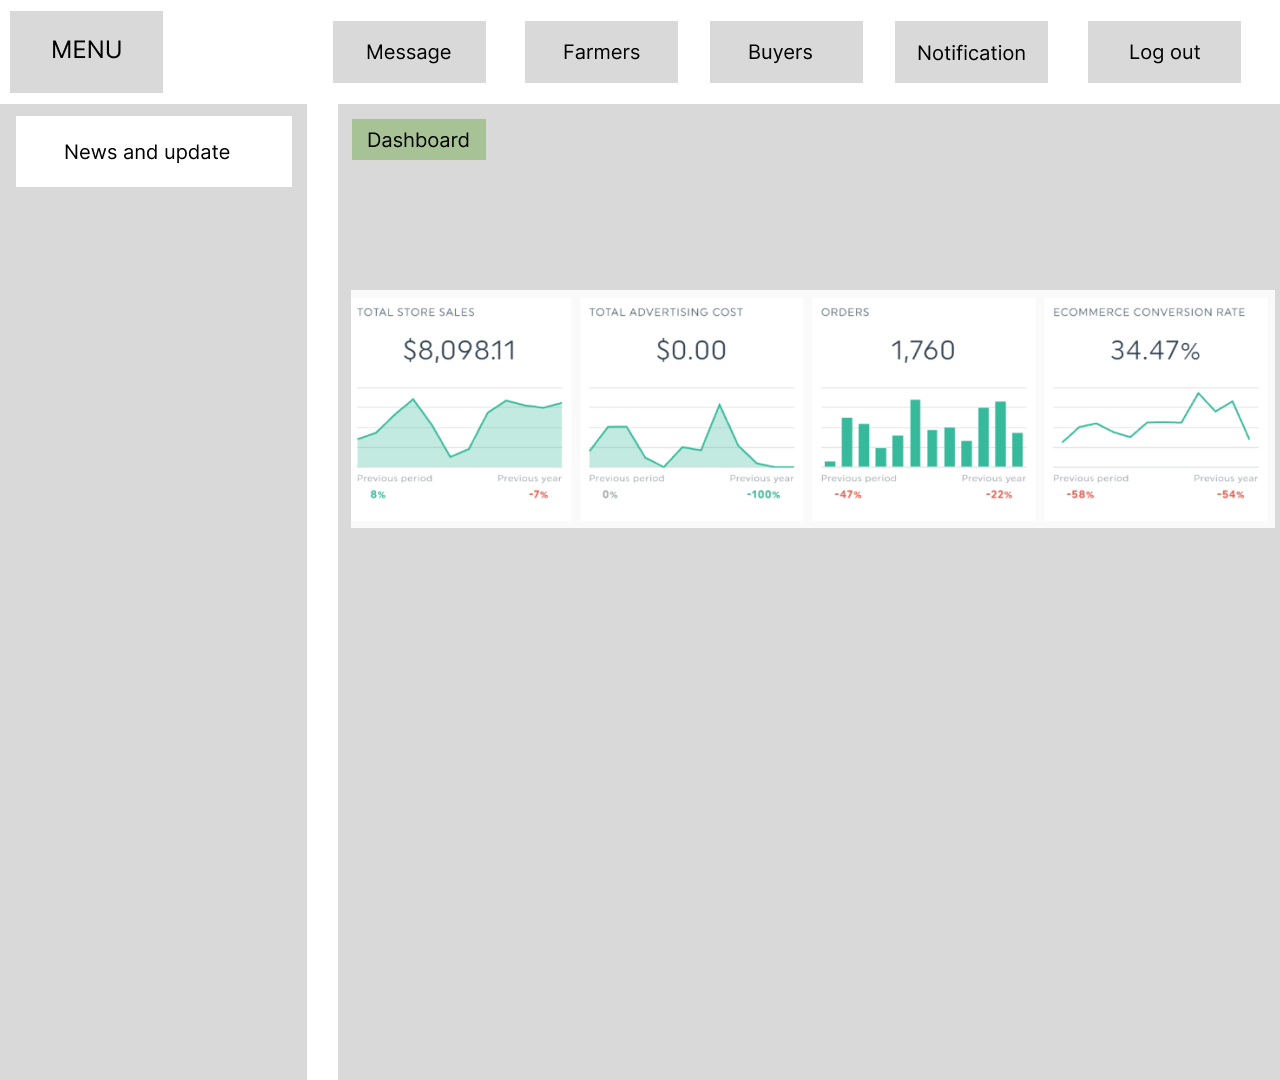
\includegraphics[width=0.9\textwidth]{Texfiles/images/wireframe/2.2 DA Home Page.png}
    \caption{Agriculture Officer Home Page}
    \label{fig:agri-home}
\end{figure}

Figure~\ref{fig:agri-home} shows the agriculture officer dashboard. The main area presents summary tiles with key indicators such as the number of registered farmers, active crop listings, available produce by category, pending resource requests, and recent system activity. These indicators help agriculture personnel monitor crop availability, farmer participation, and support needs within the municipality.

\subsubsection{Agriculture Officer Farmers Page}

\begin{figure}[htbp]
    \centering
    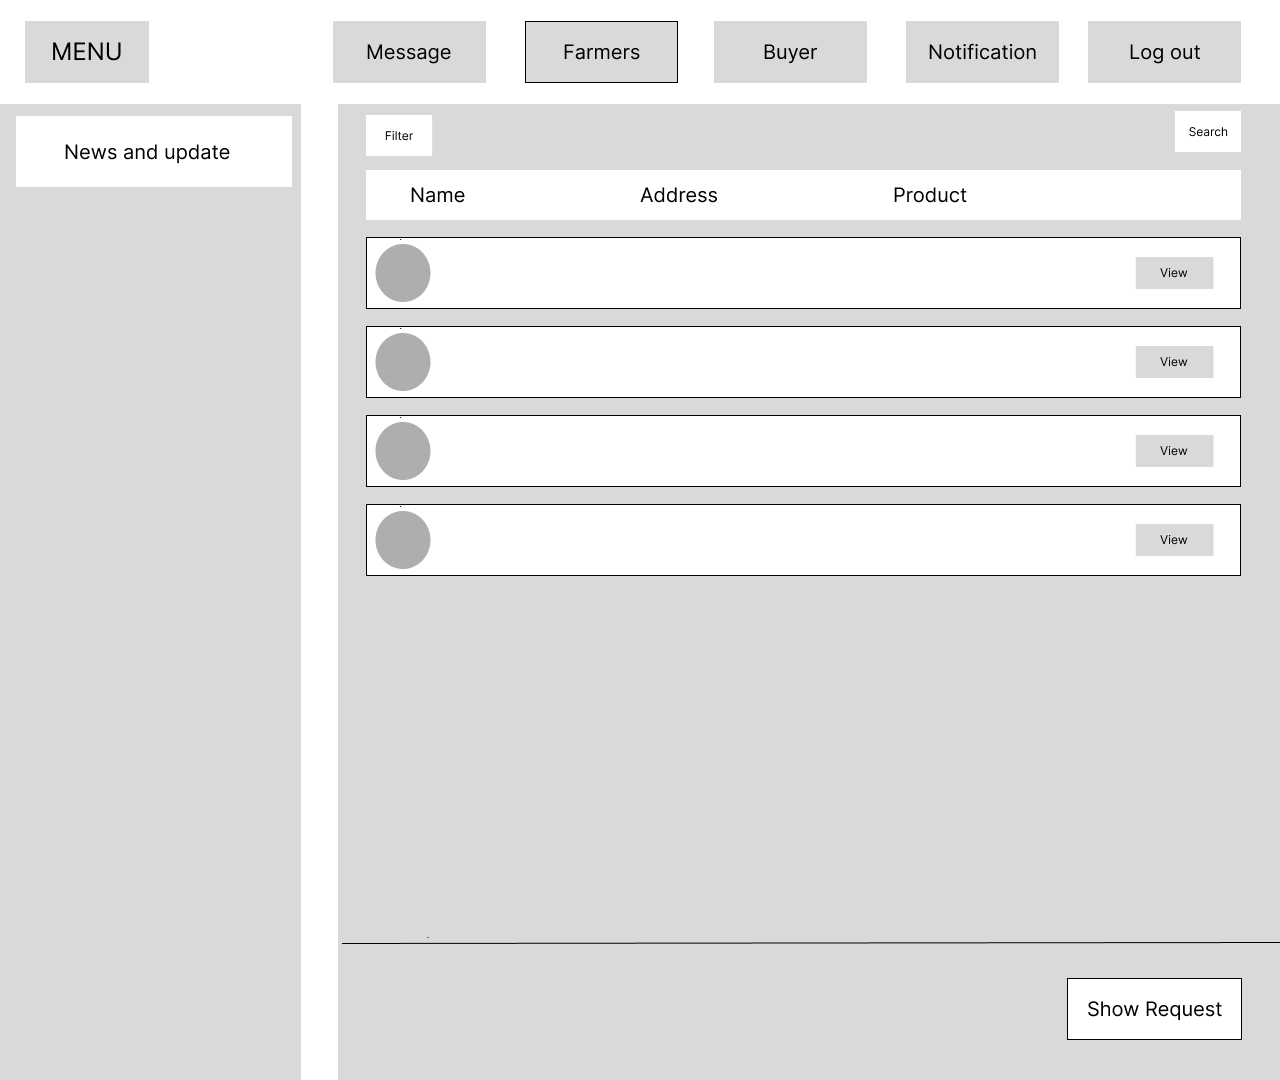
\includegraphics[width=0.9\textwidth]{Texfiles/images/wireframe/3. DA Farmer.png}
    \caption{Agriculture Officer Farmers Page}
    \label{fig:agri-farmers}
\end{figure}

Figure~\ref{fig:agri-farmers} shows the agriculture officer farmers page, which lists registered farmers. Columns include the farmer's name, address, and posted products. Each row has a \emph{View} button to open the farmer's profile and details. A \emph{Filter} button and search box allow agriculture personnel to find farmers based on criteria such as name or location. The \emph{Show Request} button displays pending requests from farmers, such as requests for agricultural assistance.

\subsubsection{Agriculture Officer Buyers Page}

\begin{figure}[htbp]
    \centering
    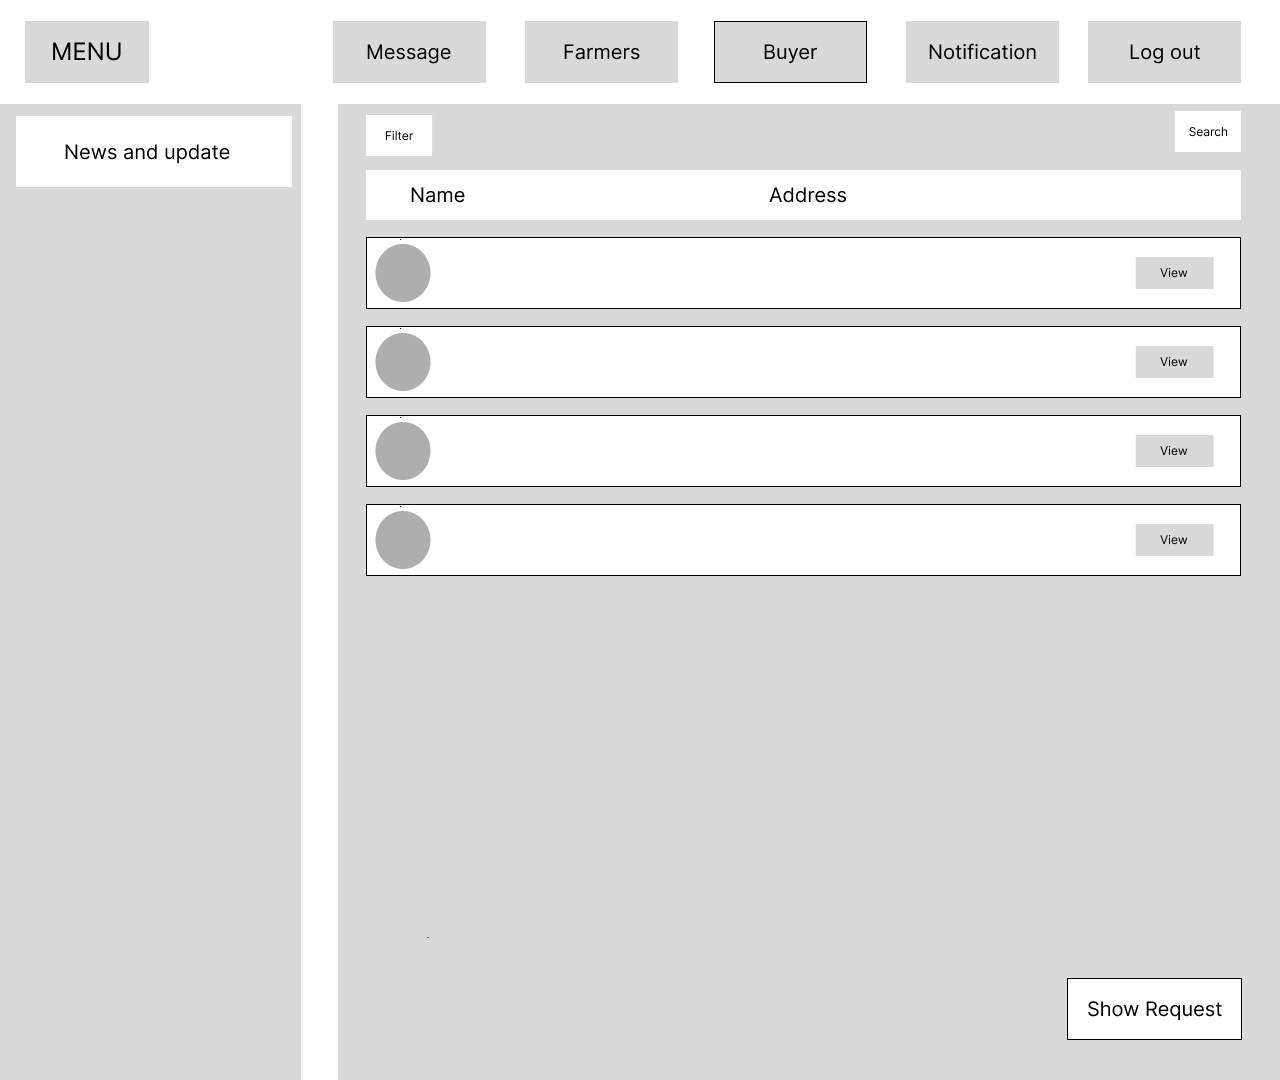
\includegraphics[width=0.9\textwidth]{Texfiles/images/wireframe/3.1 DA Buyer.png}
    \caption{Agriculture Officer Buyers Page}
    \label{fig:agri-buyers}
\end{figure}

Figure~\ref{fig:agri-buyers} shows the agriculture officer buyers page, which has a structure similar to the farmers page but is intended for buyer records. It lists the name and address of each buyer, with a \emph{View} button to inspect the buyer's profile. The filter and search tools support the monitoring of buyer registrations and related records.

\subsubsection{Message Page}

\begin{figure}[htbp]
    \centering
    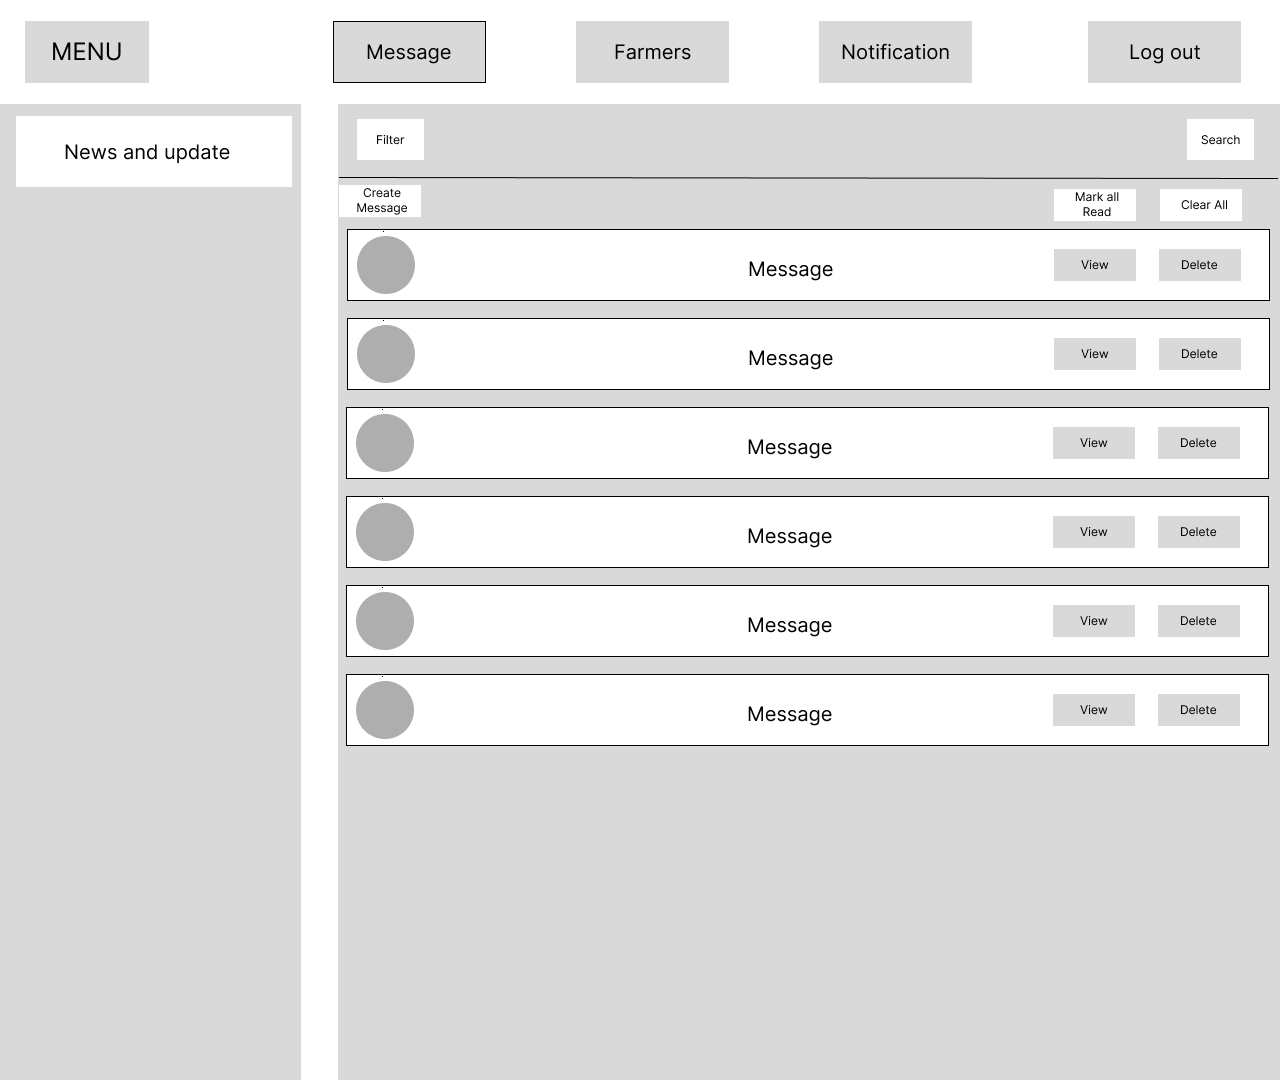
\includegraphics[width=0.9\textwidth]{Texfiles/images/wireframe/4. Message.png}
    \caption{Message Page}
    \label{fig:message-page}
\end{figure}

Figure~\ref{fig:message-page} shows the messaging page used for communication between users, such as farmer-to-buyer or farmer-to-agriculture officer communication. The page includes tools for filtering, searching, viewing, marking messages as read, and deleting messages. A create message function allows users to start a new conversation.

\subsubsection{Notification Page}

\begin{figure}[htbp]
    \centering
    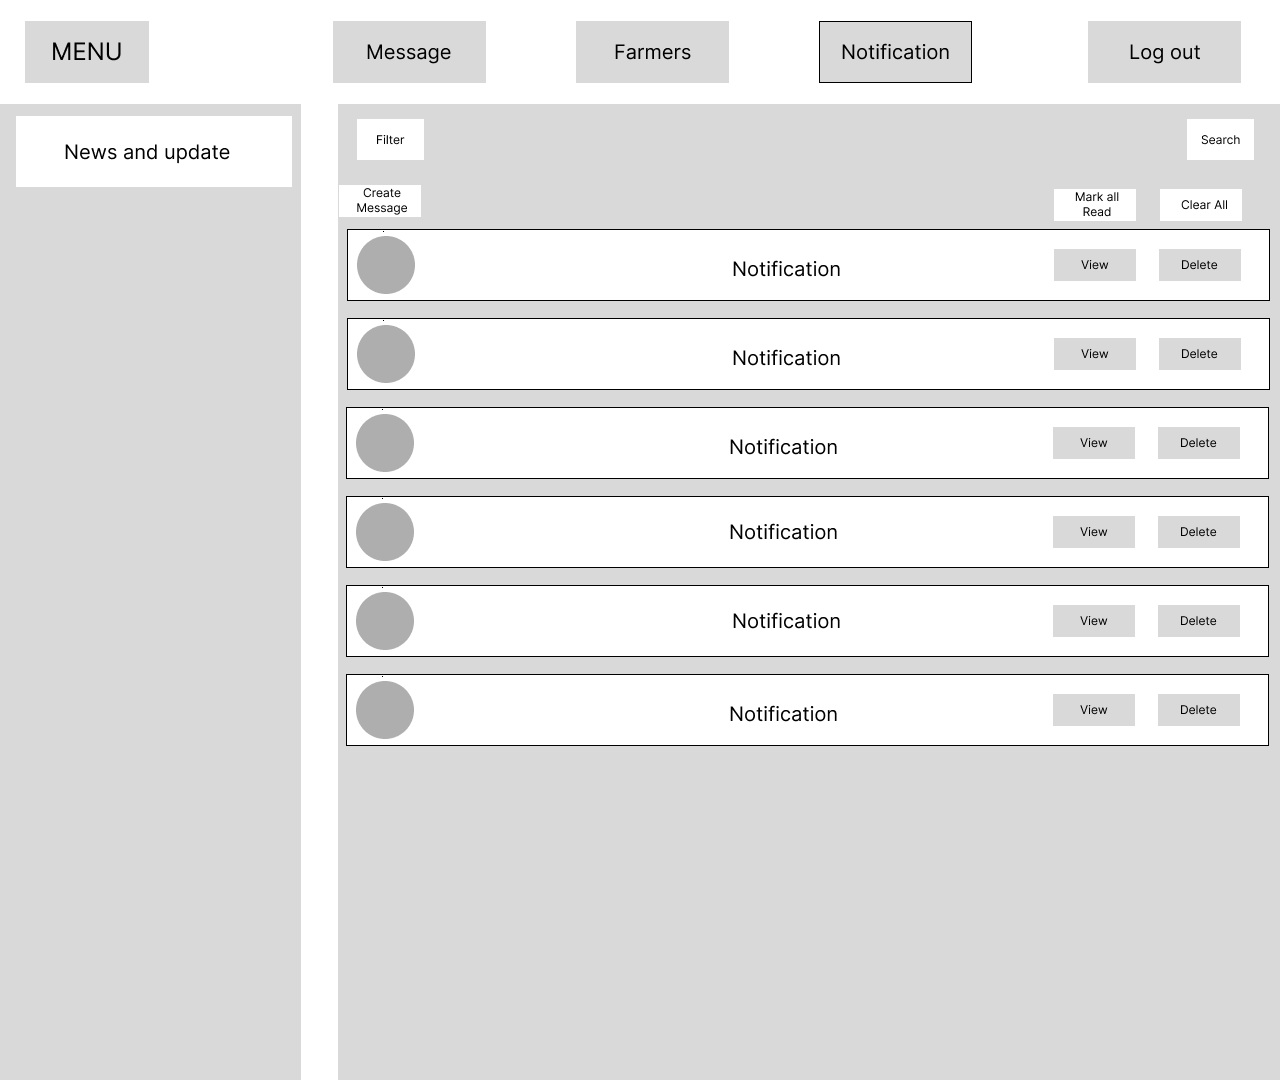
\includegraphics[width=0.9\textwidth]{Texfiles/images/wireframe/5. Notification.png}
    \caption{Notification Page}
    \label{fig:notification-page}
\end{figure}

Figure~\ref{fig:notification-page} shows the notifications page. This page displays system alerts such as approved requests, new messages, announcements, and other important updates. Users can view notification details, mark notifications as read, search, filter, or delete notifications. For important agriculture-related updates, the system can also send SMS alerts to selected users.

\subsection{Materials/Technologies Used}

The system was built using a PHP and MySQL stack suitable for shared hosting and local government or community-level deployment. The selected technologies were chosen because they are widely supported, relatively low-cost, and appropriate for organizations operating with limited infrastructure and budget.

\subsubsection*{Backend Runtime and Framework}

\begin{itemize}
    \item \textbf{PHP 8.x} was used as the primary backend runtime.
    
    \item \textbf{Flight microframework} was used to handle routing and controller dispatch. Routes are defined with \verb|Flight::route| and mapped to controller functions responsible for processing requests and rendering responses.
    
    \item \textbf{Composer} was used to manage dependencies and PSR-4 autoloading, helping keep the codebase organized and maintainable.
\end{itemize}

\subsubsection*{Frontend Technologies}

\begin{itemize}
    \item The user interface was built using \textbf{HTML5}, \textbf{CSS}, \textbf{JavaScript}, and \textbf{Bootstrap 5}.
    
    \item Bootstrap's grid system and components were used to create responsive forms, tables, and cards that adapt to different screen sizes, from smartphones to desktop monitors.
    
    \item Basic accessibility practices were applied, including descriptive labels, logical tab order, readable text, sufficient visual contrast, clear icons, and simplified interface elements.
\end{itemize}

\subsubsection*{Localization and Notification Support}

\begin{itemize}
    \item The system includes a \textbf{Bisaya language toggle} that allows users to switch selected interface labels, instructions, and messages into Bisaya. This feature supports farmers and local users who are more comfortable using the local language.
    
    \item The system supports \textbf{SMS notifications} for important updates such as resource request status, advisories, and official agriculture-related announcements. This feature helps reach farmers who may have limited internet access or who do not regularly check the web application.
\end{itemize}

\subsubsection*{Database}

\begin{itemize}
    \item A \textbf{MySQL} database was used to store structured data for users, roles, product categories, product listings, messages, notifications, resource requests, language-related records, SMS notification records, and audit logs.
    
    \item Tables were indexed on commonly searched fields such as product name, category, and barangay to support efficient filtering and search.
    
    \item Foreign keys and constraints were used where appropriate to maintain referential integrity among related records.
\end{itemize}

\subsubsection*{Development Tools}

\begin{itemize}
    \item A PHP-compatible code editor or integrated development environment was used for system development.
    
    \item Git was used to manage source code versions and track changes during development.
    
    \item Simple task lists or lightweight project management tools were used to monitor feature implementation, bug fixing, and documentation progress.
\end{itemize}

\subsection{System Design}

The system design covers both the functional and non-functional aspects of the application. Functional design describes the main features and modules of the system, while non-functional design describes system qualities such as usability, performance, security, availability, and maintainability.

\subsubsection*{Functional Design}

The main functional components of the system are:

\begin{itemize}
    \item \textbf{User Management and Roles} -- Users can register and log in, with access restricted based on their role as farmer, buyer, agriculture officer, or administrator. Each role has access to role-specific menus, pages, and functions.
    
    \item \textbf{Product Categories and Listings} -- Farmers can create, edit, view, and archive product listings. Each listing contains fields such as crop name, category, quantity, unit, price, image, barangay, status, and harvest information. Categories are managed to support consistent filtering and organization.
    
    \item \textbf{Buyer Search and Discovery} -- Buyers can browse and search for products using filters such as category, crop name, location, price range, and availability. Search results help buyers locate available produce and identify farmers to contact.
    
    \item \textbf{Messaging and Inquiries} -- The messaging module allows buyers, farmers, and agriculture personnel to send and receive messages. This supports communication related to product inquiries, resource requests, and other system-related concerns.
    
    \item \textbf{Resource Requests} -- Farmers can submit requests for farming support such as seeds, fertilizers, or technical assistance. Agriculture officers can review these requests, approve or reject them, add remarks, and update their status. Farmers can view updates on the status of their requests.
    
    \item \textbf{Notifications} -- The system provides notifications for important events such as new messages, request status updates, announcements, and other system alerts.
    
    \item \textbf{SMS Notification} -- The system supports SMS-based alerts for important updates such as resource request status, advisories, and agriculture-related announcements. This allows farmers to receive essential information even when they have limited internet access or are not actively using the web application.
    
    \item \textbf{Language Toggle} -- The system includes a Bisaya language toggle that allows selected interface labels, instructions, and messages to be displayed in Bisaya. This supports local users who are more comfortable understanding system instructions in their preferred language.
    
    \item \textbf{Dashboards and Metrics for Agriculture Officers} -- Agriculture officers can view dashboard summaries such as total active listings, available produce by category, number of registered farmers and buyers, and status of resource requests. These summaries support basic monitoring and decision-making.
    
    \item \textbf{CSV Export} -- Authorized users can export filtered product listing records to a CSV file. This supports offline review, documentation, and reporting by agriculture personnel.
    
    \item \textbf{Validation, Feedback, and Logging} -- Server-side validation is applied to important forms. User-friendly messages are displayed when actions succeed or fail. Basic logging is implemented for key actions to support troubleshooting and accountability.
\end{itemize}

\subsubsection*{Non-Functional Design}

Several non-functional qualities were considered in the design and implementation of the system:

\begin{itemize}
    \item \textbf{Usability and Accessibility} -- Screens were designed to be simple and easy to understand, with clear labels, consistent navigation, and minimal required fields. The interface was designed to work on mobile and desktop browsers to support users with different devices and levels of digital literacy. The system also includes a Bisaya language toggle to make selected labels and instructions easier to understand for local users. In addition, SMS notifications support accessibility by allowing farmers to receive important updates even when internet access is limited.
    
    \item \textbf{Performance} -- Page templates, database queries, and commonly searched fields were organized to support acceptable performance on shared hosting. Unnecessary data loading was minimized to keep response times reasonable.
    
    \item \textbf{Security} -- The system uses SHA 256 for encrypted communication. Passwords are stored using secure hashing mechanisms. Role-based access checks are enforced on protected routes. Input validation, prepared statements, and output escaping are used to reduce risks such as SQL injection and cross-site scripting.
    
    \item \textbf{Availability and Backup} -- The system uses hosting-level backup and monitoring features to support data recovery and availability. This helps reduce the risk of data loss in case of technical failure.
    
    \item \textbf{Maintainability} -- The project uses organized folders, consistent naming, and separation of configuration from application code. This structure supports future updates, bug fixes, and possible system expansion.
\end{itemize}

\subsection{Implementation}

\begin{figure}[htbp]
    \centering
    \vspace{4ex}
    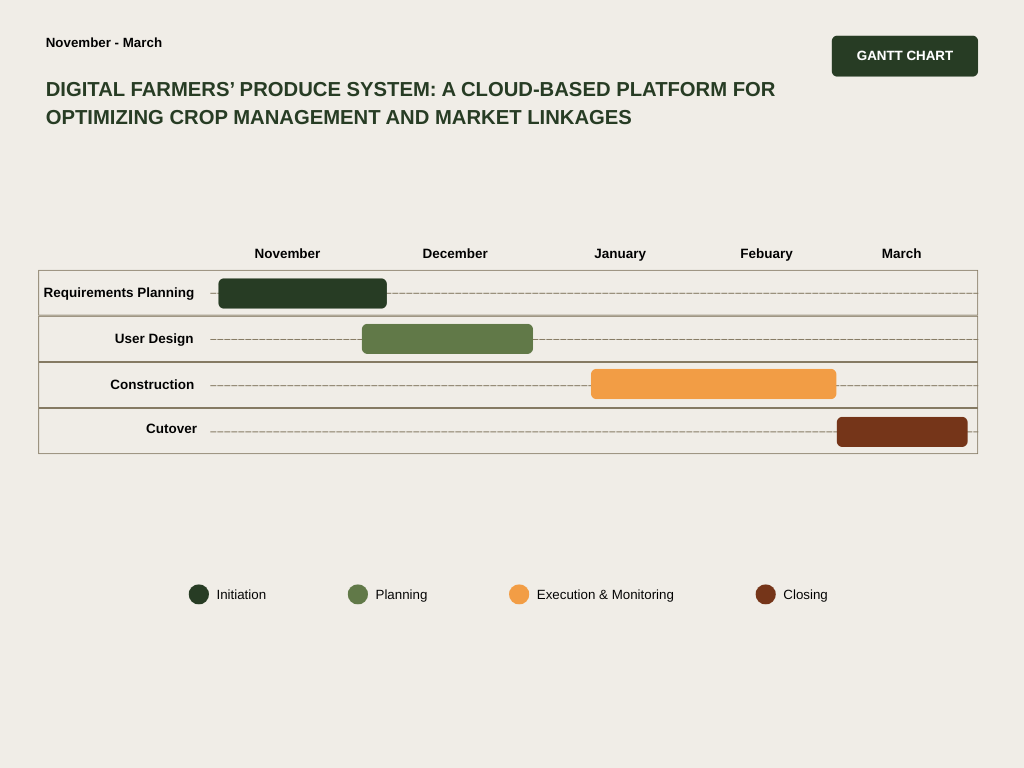
\includegraphics[width=0.9\textwidth]{Texfiles/images/gannt.png}
    \caption{Gantt Chart}
    \label{fig:gantt-chart}
\end{figure}

Figure~\ref{fig:gantt-chart} shows the project implementation schedule from November to March. The project began with the Requirements Planning phase in November, which included project initiation, planning, stakeholder interviews, document collection, and review of related literature from November~1--27. This phase helped establish the project problem, user needs, system requirements, and initial documentation.

The User Design phase followed from late November through December. During this phase, the gathered information was analyzed, the system outline was prepared, and the wireframes, user flows, and documentation drafts were created. Revisions were made based on review and feedback before proceeding to the construction phase.

The Construction phase was conducted in January and February. This phase covered the development of the core system modules, including user management, produce listing, buyer search, messaging, notifications, SMS alerts, resource requests, dashboard summaries, Bisaya language toggle, and CSV reporting. Testing and bug fixing were also performed during this period to improve functionality, usability, and reliability.

During implementation, additional accessibility and communication features were included to support the local farming context. A Bisaya language toggle was added to help users understand selected system labels and instructions in the local language. SMS notification support was also implemented to send important updates, such as resource request status and advisories, to farmers who may have limited internet access.

The Cutover phase was scheduled from late February to March. This phase included pilot deployment, user orientation, user testing, security testing, User Acceptance Testing based on the Technology Acceptance Model (TAM), review of results, final documentation, and preparation for the final defense and submission of requirements.